% !TEX root = WWW.tex
\section{Experimental Study}

We now  perform an experimental evaluation of our labeling scheme on a number of power-law networks.
The source code for our experiments can be found at:\\ \url{www.diku.dk/\~simonsen/suppmat/podc15/powerlaw.zip}

\subsection{Experimental Framework}\label{Sec:Experimental}
\paragraph{Performance Indicators}
Recall that our labeling scheme separates  the nodes according to a selected threshold from the range $0 \dots n$, which we select as a function of  the power-law parameter $\alpha$.
The following observation is the key to assess our labeling scheme's quality.
Suppose we chose a threshold  $n_0$ for a graph $G$, and call  the maximum label size of a thin node, $T(n_0)$ and the maximum label size of a fat node $F(n_0)$.  The size of our labeling scheme for the graph $G$ is the larger of these two values.
The critical observation is that, as our selection of threshold $n_0$ increases, $T(n_0)$ monotonically increases and  $F(n_0)$ monotonically decreases.
Our strategy thus arrives to optimality if we choose $n_0$ that minimises  the value $F(n_0)-T(n_0)$, in other words, where the curves of both functions intersect.
In the remainder of this section we call such threshold the \emph{empirical} threshold.

In contrast, we set the threshold in our labeling scheme as $\lceil \sqrt[\alpha]{C n/(\alpha-1)} \rceil$, which we denote as the \emph{predicted} threshold.
It is an approximation to the theoretically optimal threshold choice when degree distributions follow the power-law curve $k\mapsto Cn/k^\alpha$ perfectly, using integration as used in Proposition~\ref{prop:Contained}.

%We set up the following performance indicators to measure (i) the difference in label size with predicted and empirical threshold, and (ii) the label size obtained by our labeling scheme on several data sets, compared to other labeling schemes.

\emph{Performance Indicator i:} We measure the label sizes for the labeling schemes with the predicted and empirical thresholds. We interpret a small relative difference between these label sizes means that the predicted threshold can achieve small label sizes without examining the global properties of the network other than the power-law parameter $\alpha$. 
 
\emph{Performance Indicator ii:} We  compare the label sizes attained by our labeling schemes to other labeling schemes, namely state-of-the art labeling schemes for the classes of bounded-degree, sparse and general graphs using the  labeling schemes suggested in \cite{adjiashvili2014labeling},  Theorem~\ref{sparse-label} and \cite{alstrup2014adjacency}.  We interpret small label sizes for our scheme, especially in comparison with ``small'' classes like the class of bounded-degree graphs, as a sign that our labeling scheme efficiently utilizing  the extra information about the graphs: namely that their degree distribution is reasonably well-approximated by a power-law.


\emph{Performance Indicator iii:}
The threshold can be selected from $0$ to the maximum degree.
 We measure  difference between the predicted and empirical threshold in percentages with respect to the maximum degree.
This best captures how close our ''guess" of the right threshold was.
 
 %\footnote{Additional notes on these values are found in Appendix~\ref{Section:TotalStorage}.

\paragraph{Test Sets}
We employ both real-world and synthetic data sets. 

The six \emph{synthetic} data sets are created by first generating a power-law degree sequence using the method of Clauset et al.~\cite[App.\ D]{clauset2009power}, subsequently constructing a corresponding graph for the sequence using the Havel-Hakimi method~\cite{hakimi1962realizability}. 
We use the range $2< \alpha < 3$ as suggested in~\cite{clauset2009power} as this range of $\alpha$ occurs most commonly in modeling of real-world networks. We generate graphs of $300,000$ and $1M.$ vertices denoted  s300$^{\alpha=x}$  and s1M$^{\alpha=x}$  respectively, for $x \in \{2.2,2.4,2.6,2.8\}$. 


The three \emph{real-world} data sets originate  from articles that found the data to be well-approximated by a power-law. 
The \textsc{www} data set  \cite{albert1999internet} contains information on links between webpages within the nd.edu domain. 
The \textsc{enron} data set ~\cite{leskovec2009community}  contains email communication between  Enron employees (vertices are email addresses; there is a link between two addresses
if a mail has been sent between them).
The \textsc{internet} data set~\cite{newman} provides a snapshot the Internet structure at the level of  autonomous systems, reconstructed from BGP tables. 
For all of these sets, we consider the underlying simple, undirected graphs. For each set, standard maximum likelihood methods were used to compute the parameter
$\alpha$ of the best-fitting power-law curve \cite{clauset2009power}. Additional information on the data sets can be found in Table~\ref{t:datasets}.

\begin{table}[!ht]
\centering
\small
\begin{tabular}{lccccl}\hline
\multicolumn{6}{c}{Real-Life}\\\hline
Data set  & $\vert V \vert$ & $\vert E\vert$ & $\alpha$  & $\Delta_{\max}$ & Source\\\hline
\textsc{www}      & 325,729        & 1,117,563     & 2.16 & 10,721            & \cite{albert1999internet}\\
\textsc{enron}    &  36,692        &   183,830      & 1.97    &1,383         & \cite{leskovec2009community}\\
\textsc{internet} &  22,963        &    48,436      & 2.09     & 2,390        & \cite{newman}\\\hline

\multicolumn{6}{c}{Synthetic}\\\hline
s1M$^{\alpha=2.4}$    & 1,000,000       & 1,127,797      & 2.4    & 42,683 &-- \\
s1M$^{\alpha=2.6}$    & 1,000,000       & 878,472        & 2.6    & 12,169 &-- \\
s1M$^{\alpha=2.8}$    & 1,000,000       & 751,784         & 2.8   & 1,692  &-- \\
s300$^{\alpha=2.2}$    & 300,000        & 491,926        & 2.2    & 10,906 & --\\
s300$^{\alpha=2.4}$    & 300,000        & 327,631        & 2.4    & 3,265 & --\\
s300$^{\alpha=2.6}$    & 300,000        & 261,949        & 2.6    & 1,410 & --\\
s300$^{\alpha=2.8}$    & 300,000        & 227,247        & 2.8    & 1,842 & --\\\hline
\end{tabular}
\caption{Data sets and their properties. All graphs are undirected and simple. $\Delta_{\max}$ is the maximum degree of any vertex in the data set.}
\label{t:datasets}
\end{table}


\subsection{Findings}
Figure \ref{fig:findings} shows the distribution of maximum label sizes for one synthetic and one real-world data set. The maximum label size
for the predicted and empirical thresholds as well as upper bounds on the label sizes from different label schemes in the literature can be seen in Table \ref{t:labelsizes} for two synthetic
data sets and all three real-world data sets. 
%Plots for the remaining data sets can be found in Appendix~\ref{App:ExpRes}.


\begin{figure*}[!ht]
\centering
\subfloat[\small syn300$^{\alpha=2.2}$]{
    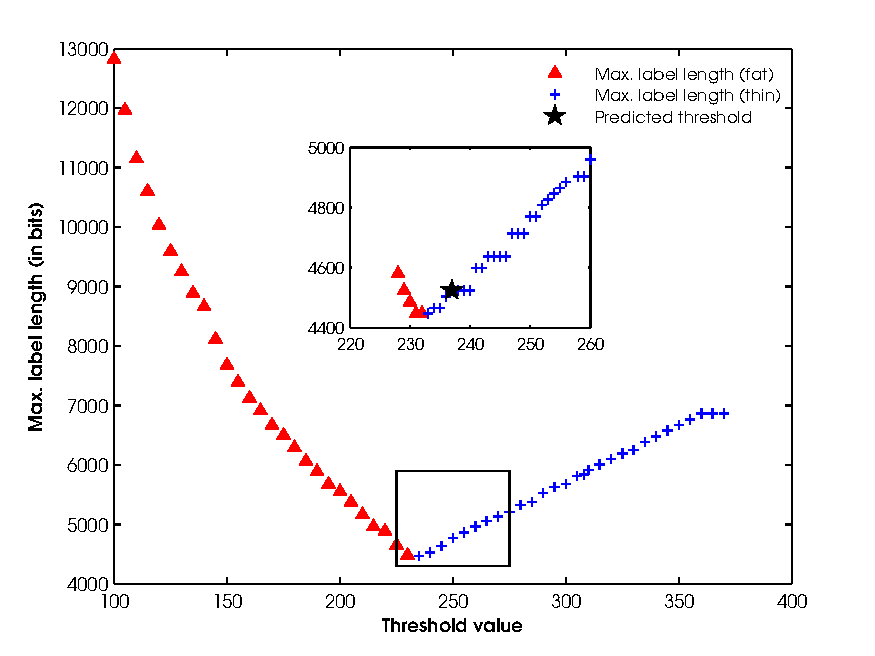
\includegraphics[width=0.4\textwidth]{Figures/synthetic-300k-alpha22.pdf}
    \label{f:fsyn300k}
}\hspace*{-2.5em}
\subfloat[\small \textsc{enron}]{
    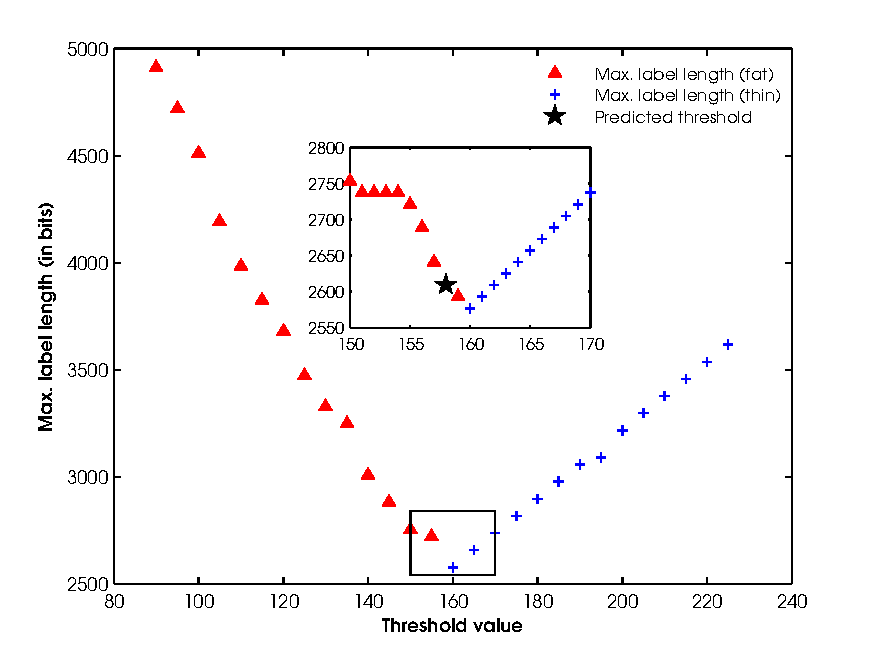
\includegraphics[width=0.4\textwidth]{Figures/enron-mail.pdf}
    \label{f:fenron}
}%
\caption{Maximum label sizes of different threshold values for the   syn300$^{\alpha=2.2}$ and \textsc{enron} data sets.
% Fat vertices are shown as red triangles and thin vertices as blue crosses.The black pentagram is the \emph{predicted} maximum label size.The transition between fat and thin vertices is the \emph{empirical} best maximum label size.
%Fig.\ \ref{f:fsyn300k} shows the syn300$^{\alpha=2.2}$ dataset, Fig.\ \ref{f:fenron} the \textsc{enron} dataset. 
The triangles and crosses represent that for the tested threshold the largest label belong to fat, resp. thin node. The star indicate the position of the predicted threshold.}
\label{fig:findings}%
\end{figure*}

Table~\ref{t:labelsizes}  shows  the maximum label sizes achieved using different labeling schemes on our data sets. ``Predicted'' shows the experimental maximum label size obtained by running our scheme on the graphs, ``Empirical'' is the label size attained by using the empirical threshold. The remaining columns show non-experimental upper bounds for different label schemes: ``Bound'' is the upper bound guaranteed in Theorem~\ref{prop:labelingMain}, ``$C$-sparse'' is  the labeling scheme for sparse graphs defined in Theorem~\ref{sparse-label}, ``BD'' is the $\lceil \frac{\Delta}{2} \rceil \lceil \log n\rceil$ bounded degree graph  labeling of~\cite{adjiashvili2014labeling}, and AKTZ is the $\lceil n/2\rceil+6$ general graph  labeling of~\cite{alstrup2014adjacency}.
Both ``Empirical'' and  ``Bound'' using simple concatenation of labels to represent the fat bit string\footnote{Our labeling schemes introduced in this paper all make use of a succinctly represented ``fat bit string''; for our experiments, we use simple concatenation of labels instead of a bit string; this incurs a $(\log n)/\alpha$ factor on the label size, but simplifies the implementation.}.
 

\begin{table*}
\small
\begin{tabular}{ccccccccc}
Data set&Predicted &Empirical & Label Diff. & Threshold Diff.   & Upper-Bound     &$C$-sparse &Bounded Degree \cite{adjiashvili2014labeling} &AKTZ \cite{alstrup2014adjacency}\\\hline
s1M$^{\alpha=2.4}$  &$4,841$    &$4,821$  & $0.4\%$ & $0.002\%$  & $25,012 $ &$30,079$     &$426,820$ &$500,006$\\\hline
s1M$^{\alpha=2.6}$  &$3,361$    &$3,201$   & $4.8\%$ & $0.08\%$  & $15,282 $ &$26,551$     &$121,680$ &$500,006$\\\hline
s1M$^{\alpha=2.8}$  &$2,101$    &$2,061$    & $2\%$ & $0.17\%$  & $10,081 $ &$24,566$     &$16,920$  &$500,006$\\\hline
s300$^{\alpha=2.2}$ &$4,523$    &$4,447$  & $1.7\%$ & $0.05\%$  & $24,878 $ &$18,885$     &$103,607$ &$150,006$\\\hline
s300$^{\alpha=2.4}$ &$2,775$    &$2,680$   & $3.5\%$  & $0.3\%$ & $14,404 $ &$15,420$     &$31,008$  &$150,006$\\\hline
s300$^{\alpha=2.6}$ &$1,958$    &$1,920$  & $3.1\%$ & $0.35\%$   & $9,151 $  &$13,792$     &$13,395$  &$150,006$\\\hline
s300$^{\alpha=2.8}$ &$1,350$    &$1,312$  & $2.8\%$ & $0.1\%$   & $6,244 $  &$12,849$     &$17,499$  &$150,006$\\\hline
\textsc{www}        &$5,245$    &$3,060$  & $41.7\%$  & $1\%$  & $29,225 $ &$28,445$     &$101,840$ &$162,870$ \\\hline
\textsc{enron}      &$2,609$    &$2,577$  & $1.3\%$ & $0.2\%$   & $15,835 $ &$9,735$      &$11,056$  &$18,352$\\\hline
\textsc{internet}   &$1,426$    &$1,156$  & $19.0\%$  & $0.8\%$  & $8,181 $  &$4,700$      &$17,925$  &$11,487$\\\hline 
\end{tabular}
\caption{Label size in bits of labeling schemes. The two leftmost columns are experimental results with an additional difference column following; the Threshold Diff. column is the report of performance indicator iii, and the remaining are upper bounds on label sizes computed from the characteristics of the data sets.}
\label{t:labelsizes}
\end{table*}

Our findings are as follows. For Performance Indicator (i), our labeling scheme obtains maximum label size at most 3.5\% larger than what would have been obtained by using the empirical threshold for all synthetic data sets.
This is expected---the synthetic data sets are graphs generated specifically to have power-law distributed degree distribution. For the real-world data sets, the labeling scheme
obtains maximum label size at most 41.7\% larger than by using the empirical threshold; this larger deviation is likely due to degree distributions of the data sets being close to, but not quite,
power-law distributions due to natural phenomena or noise. E.g., for the \textsc{enron} data set there is sudden drop in frequency between nodes of degree $< 158$ and $\geq 158$.

For Performance Indicator (ii), both our experimental results and theoretical upper bounds for our labeling scheme are several orders of magnitudes lower than for labeling schemes aimed at more general classes of graphs, as expected. Of the more general classes of graphs, it is most interesting to compare the upper bound of bounded degree graphs---the most restrictive class of graphs that both contains the class of power-law graphs and has an efficient labeling scheme described in the literature~\cite{adjiashvili2014labeling}. As seen in Table \ref{t:labelsizes}, the upper bound on our labeling schemes for both power-law graphs and sparse graphs have better upper bounds on label sizes, but only marginally so for data sets with low maximum degree and low values of the power-law parameter $\alpha$, e.g. \textsc{Enron} ($\alpha = 1.97$). 
The actual label sizes obtained in the experiments (the two leftmost columns of Table \ref{t:labelsizes}) are substantially lower than the upper bounds, that is,
the labeling scheme performs much better in practice than suggested by theory (down to less than a kilobyte per vertex for all data sets). 
This phenomenon may be due to the degree distribution of the graphs of the data sets having only minor deviation from a power-law for small vertex degrees; our upper bounds on the label size are derived by using the very rich family $\PLB$ that allows very large deviation from a power-law for degrees between $1$ and $\sqrt[\alpha]{n/\log n} - 1$.

Finally, note that our labeling scheme supports adjacency for \emph{directed} graphs by using one more bit per edge in each label to store the edge orientation. For data sets whose natural interpretation is as a directed graph (e.g., the \textsc{www} set where edges are outgoing and incoming links), the results of Table \ref{t:labelsizes} thus carry over with just one more bit
added to the numbers in the two leftmost columns.

\section{Conclusion and Future Work}

We have devised adjacency and distance labeling schemes for sparse graphs and graphs whose degree distribution approximately follows a power-law distribution.
 We have proven lower bounds for the class of power-law graphs showing that our adjacency labeling scheme is  almost asymptotically optimal. 
 Furthermore, we have shown experimentally that the labeling scheme for power-law graphs obtain
results in practice requiring very little space (labels smaller than a kilobyte per vertex for real-world graphs with several hundreds of thousands of vertices).


\subsection{Future work}

It would be of interest to test the performance of the labeling scheme on more real-world data sets.
Our labeling schemes are designed for static networks, and it will be interesting to convert it  into a fully dynamic labeling schemes that handles insertions and deletions. We point out that this can be done easily in practice, by allowing re-labeling of fat nodes that become thin, or vice-versa. As such changes can be suppressed, it seems plausible that the label size can be maintained using very few acts of re-labeling.
Labeling schemes for power law graphs can likely be devised for the realistic case where the scheme only has incomplete knowledge of the graph, for example when the expected frequency of vertices of each degree is known, but not the exact frequency of each vertex.

As our labeling scheme can be extended to handle directed graphs by using a single bit more per label, it would be interesting to investigate the overhead incurred by distributing the storage of the graph topology to the labels (as per our labeling scheme) compared to the substantial body of work on storing directed power-law graphs directly in main memory (so-called ``web-graph compression'') \cite{guillaume2002efficient,asano2003compact, asano2008efficient,claude2010fast}.
The  label sizes attained in Sec.~\ref{Sec:Experimental} can be reduced by using the succinctly represented ``fat bit string'' as well as an additional rule that prevents storing  an edge in two  labels; doing so would yield a small multiplicative reduction in label size, making our labeling scheme even more practical. 

Lastly, the entropy of both the Chung-Liu and the BA model was recently determined to be similar. It is thus quite surprising that the label size difference is as large as we have proved. It is thus conjectured that the number of nodes of large label size is very small for this family.

